\section{Introduktion} % Claes
\subsection{Vesikler og meningen med detektionen - Cryo-EM} % Claes
En celle i nervesystemet kaldes for en neuron eller en nervecelle. En neuron er den vigtigste del i nervesystemet, der bl.a. indeholder hjernen og rygsøjlen. Nerveceller har bl.a. til opgave at modtage og sende information ved hjælp af elektriske og kemiske signaler. I en nervecelle er der så en række synaptiske vesikler, der indeholder neurotransmitters. Når en nervecelle skal sende et impulssignal til en anden nervecelle, bevæger den synaptiske vesikel sig til kanten af nervecellen og udsender neurotransmitters. Nervecellerne genskaber så de synaptiske vesikler så der igen kan sendes nye signaler. To nerveceller hvor der er markeret en synaptisk vesikel i den øverste ses i figur \ref{fig:intro_syntrans}. I den menneskelige hjerne har en synaptisk vesikel en gennemsnitlig diameter på 39.5 nanometer med en standard afvigelse på 5.1 nanometer. En af klasserne af neurotransmitters er aminosyre.  

\begin{figure}[H]
	\centering
	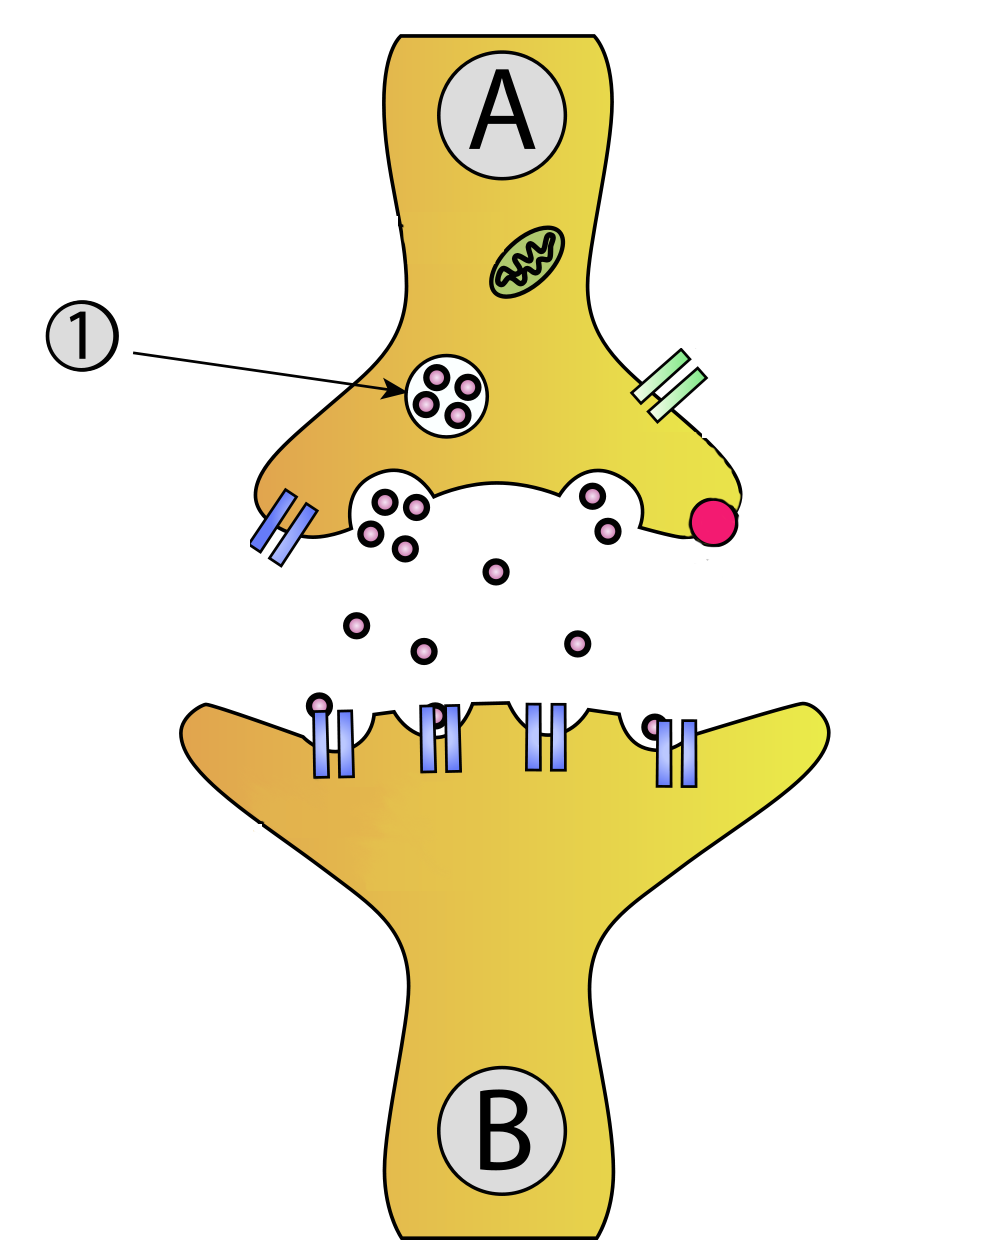
\includegraphics[scale=0.2]{files/intro/img/synTransmitter.png}
	\caption{To neuroner, en afsender af neurotransmitters (A) og en modtager (B). Pilen peger på en synaptisk vesikel.\label{fig:intro_syntrans}}
	% Original fra : http://en.wikipedia.org/wiki/File:Synapse_diag1.svg
\end{figure} 

% OBS - Clear følgende med Jon / Biologen.
Ved at se på vesiklers placering i forhold til hinanden i celler, kan man afgøre om personen er deprimeret eller ej. Igangværende forskning går i øjeblikket ud på at finde ud af hvorvidt depression er arvelig fra mor til barn, hvis moderen er deprimeret under graviditeten. Vores problem går ud på at lave et system der kan hjælpe forskerne med at detektere disse vesikler i en celle. Det videre arbejde med projektet er så at bruge denne detektion af vesikler til at analysere deres placering i forhold til hinanden, og altså automatisere hele proceduren. Vores problem går bare ud på at detektere vesiklerne.

Til at tage billeder af vesikler benyttes et Cryo-elektron mikroskop, der tager et udsnit af en hjerne og forstørrer cellerne op så de er synlige i et billede. Et cryo-elektron mikroskop tager billeder i meget lave temperaturer, hvilket er godt da cellerne er meget følsomme over for stråling, der gør at der er høj støj i billederne, hvilket også fremgår af billedet i figur \ref{fig:intro_celler}.

\begin{figure}[H]
	\centering
	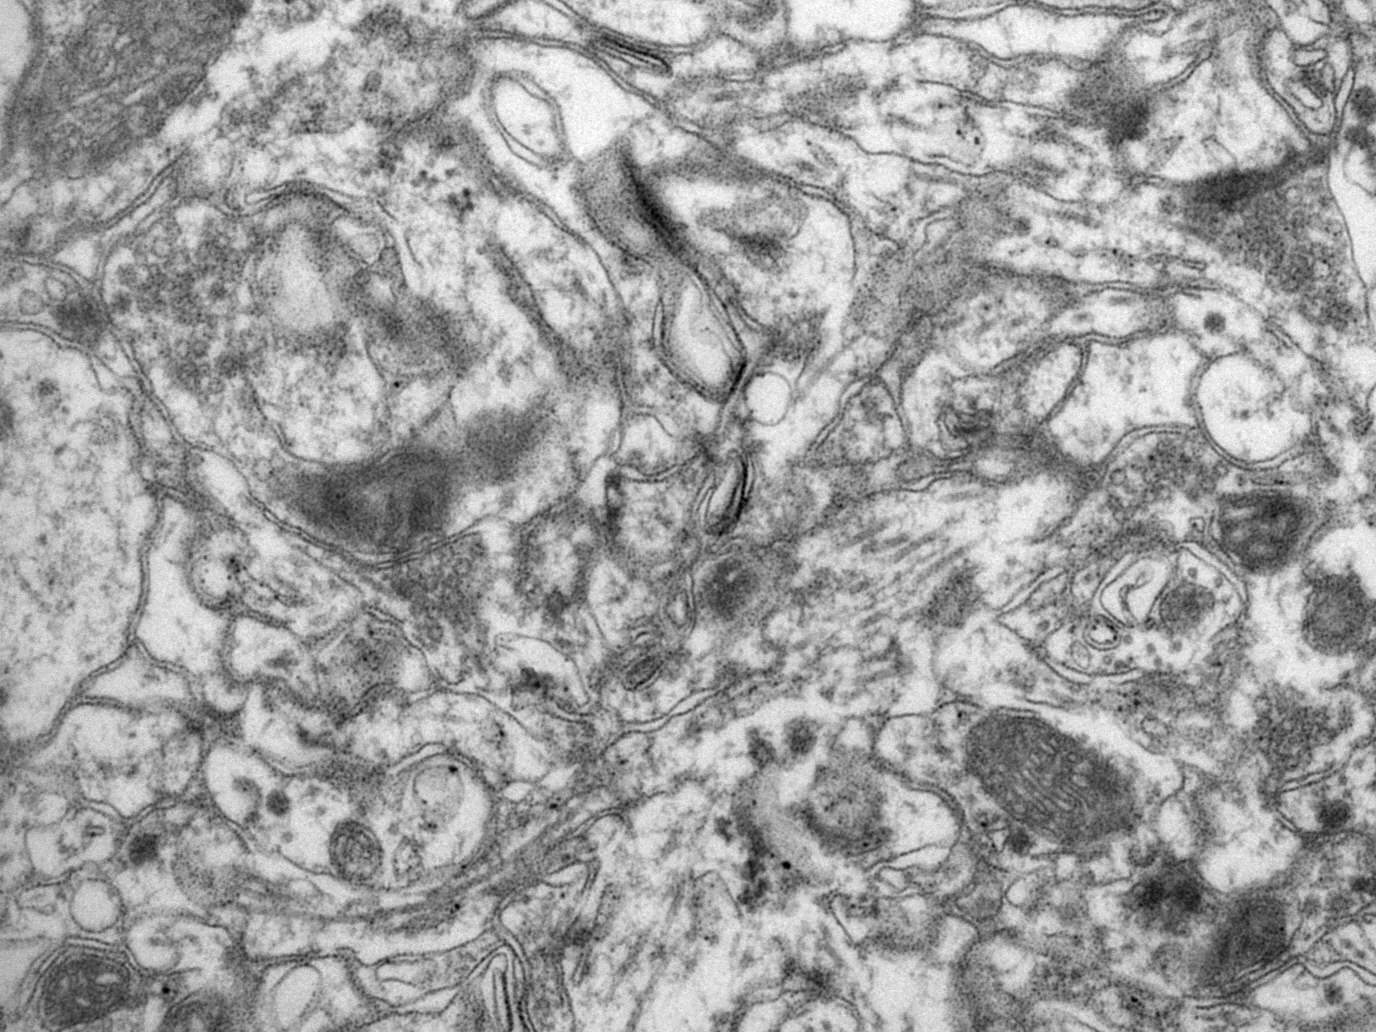
\includegraphics[scale=0.5]{files/intro/img/celler.jpg}
	\caption{Billede af nerveceller taget med et cryo-elektron mikroskop.\label{fig:intro_celler}}
\end{figure}

\subsection{Ground truth}									% Claes
Vi er ude efter at detektere synaptiske vesikler i celler, og er derfor kun interesseret i billeder der indeholder en enkelt celle. Billedet i figur \ref{fig:intro_celle} viser et sådan udsnit. Grundet den høje støj omkring vesiklerne, er det svært at se hvor der er en vesikel, og hvor der bare er støj fra de omkringliggende vesikler som tilsammen ligner en ny vesikel. Derfor har vi i samarbejde med en biolog markeret ground truth i de billeder vi arbejder med. Et af disse ses i figur \ref{fig:intro_celle_groundtruth} hvor ground truth er markeret med en blå prikker i hver vesikel.

\begin{figure}[ht]
	\begin{minipage}[b]{0.5\linewidth}
		\centering
		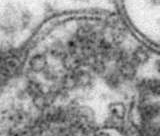
\includegraphics[scale=1.5]{files/intro/img/celle.png}
		\caption{Udsnit af en enkelt nervecelle.\label{fig:intro_celle}}
	\end{minipage}
	\hspace{0.5cm}
	\begin{minipage}[b]{0.5\linewidth}
		\centering
		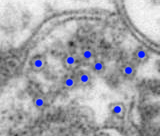
\includegraphics[scale=1.5]{files/intro/img/celle_groundtruth.png}
		\caption{Udsnit af en enkelt nervecelle med ground truth markeret.\label{fig:intro_celle_groundtruth}}
	\end{minipage}
\end{figure}
  

\subsection{Hvad ønsker vi at finde- Målsætning}			% Claes
Hvis man med sine egne øjne ikke kan skældne en støj fra en kant, kan man forestille sig at det også er svært at detektere alle vesikler korrekt ved hjælp af computeren. Man kan både komme til at vælge nogle områder der ligner en vesikel meget, men ikke er det, og omvændt kan man undlade at vælge en vesikel, da området omkring den har så meget støj at det er svært at skældne hvor kanten stopper og støjen starter. 

\begin{figure}[H]
	\centering
	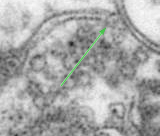
\includegraphics[scale=1.5]{files/intro/img/celle_questionves.png}
	\caption{Er der en vesikel for enden af pilen?\label{fig:intro_celle_question}}
\end{figure}

Et eksempel på et område hvor det er svært at se hvorvidt der er en vesikel eller ej, ses i figur \ref{fig:intro_celle_question}. Øverst i billedet ses to områder med paralelle linjer. Området mod venstre er kanten på cellen hvori vi ønsker at detektere vesikler. Den anden er kanten fra en anden celle der går lidt indover vores celle. Pilen peger så mod en område hvor de to kanter mødes, og der er meget støj. Det er svært at se med det utrænede øje hvorvidt dette er en vesikel eller bare støj. Yderligere er billederne taget ud fra meget tynde udsnit af hjernen, og det kan forekomme at man kan se skyggen af en vesikel eller celle der ligger over det snit man kigger på.  

Vores målsætning er derfor ikke at finde ground truth i alle billeder, uden at detektere en eneste falsk positiv vesikel. Succeskriteriet er blot at finde størstedelen af vesiklerne, og holde antallet af falske positive nede.   

%% Kildehenvisninger
% http://en.wikipedia.org/w/index.php?title=Synaptic_vesicle&oldid=422206613
% http://en.wikipedia.org/w/index.php?title=Neurotransmitter&oldid=429460993
% http://en.wikipedia.org/w/index.php?title=Neuron&oldid=427379524
% http://en.wikipedia.org/w/index.php?title=Cryogenics&oldid=428358887
% http://en.wikipedia.org/w/index.php?title=Cryo-electron_microscopy&oldid=425946253


